%=================================================================
\section{Introduction}\label{sec-intro}
The sinking of the Titanic is one of the most infamous shipwrecks in history.
n this project, we aim to build a predictive model that answers the question: “what sorts of people were more likely to survive?” using passenger data (ie name, age, gender, socio-economic class, etc).
Problem Definition: Knowing from a training set of samples listing passengers who survived or did not survive the Titanic disaster, can our model determine based on a given test dataset not containing the survival information, if these passengers in the test dataset survived or not.

\section{Exploratory Data Analysis} \label{sec-preliminaries}

There are two dataset provided for analysis. 
One dataset is titled `train.csv` and the other is titled `test.csv`.
Train.csv will contain the details of a subset of the passengers on board (891 to be exact) and importantly, will reveal whether they survived or not, also known as the “ground truth”.

The `test.csv` dataset contains similar information but does not disclose the “ground truth” for each passenger. It’s your job to predict these outcomes.

Using the patterns found in the train.csv data, we predict whether the other 418 passengers on board (found in test.csv) survived.
\begin{itemize}
\item
Categorical Features in the dataset - \textcolor{orange}{Sex, Embarked}
\item
Ordinal Features in the dataset - \textcolor{orange}{Pclass}
\item
Continuous Features in the dataset - \textcolor{orange}{Age}
\end{itemize}
\begin{figure}
  \centering
  %\selectcolormodel{rgb}
  \centerline{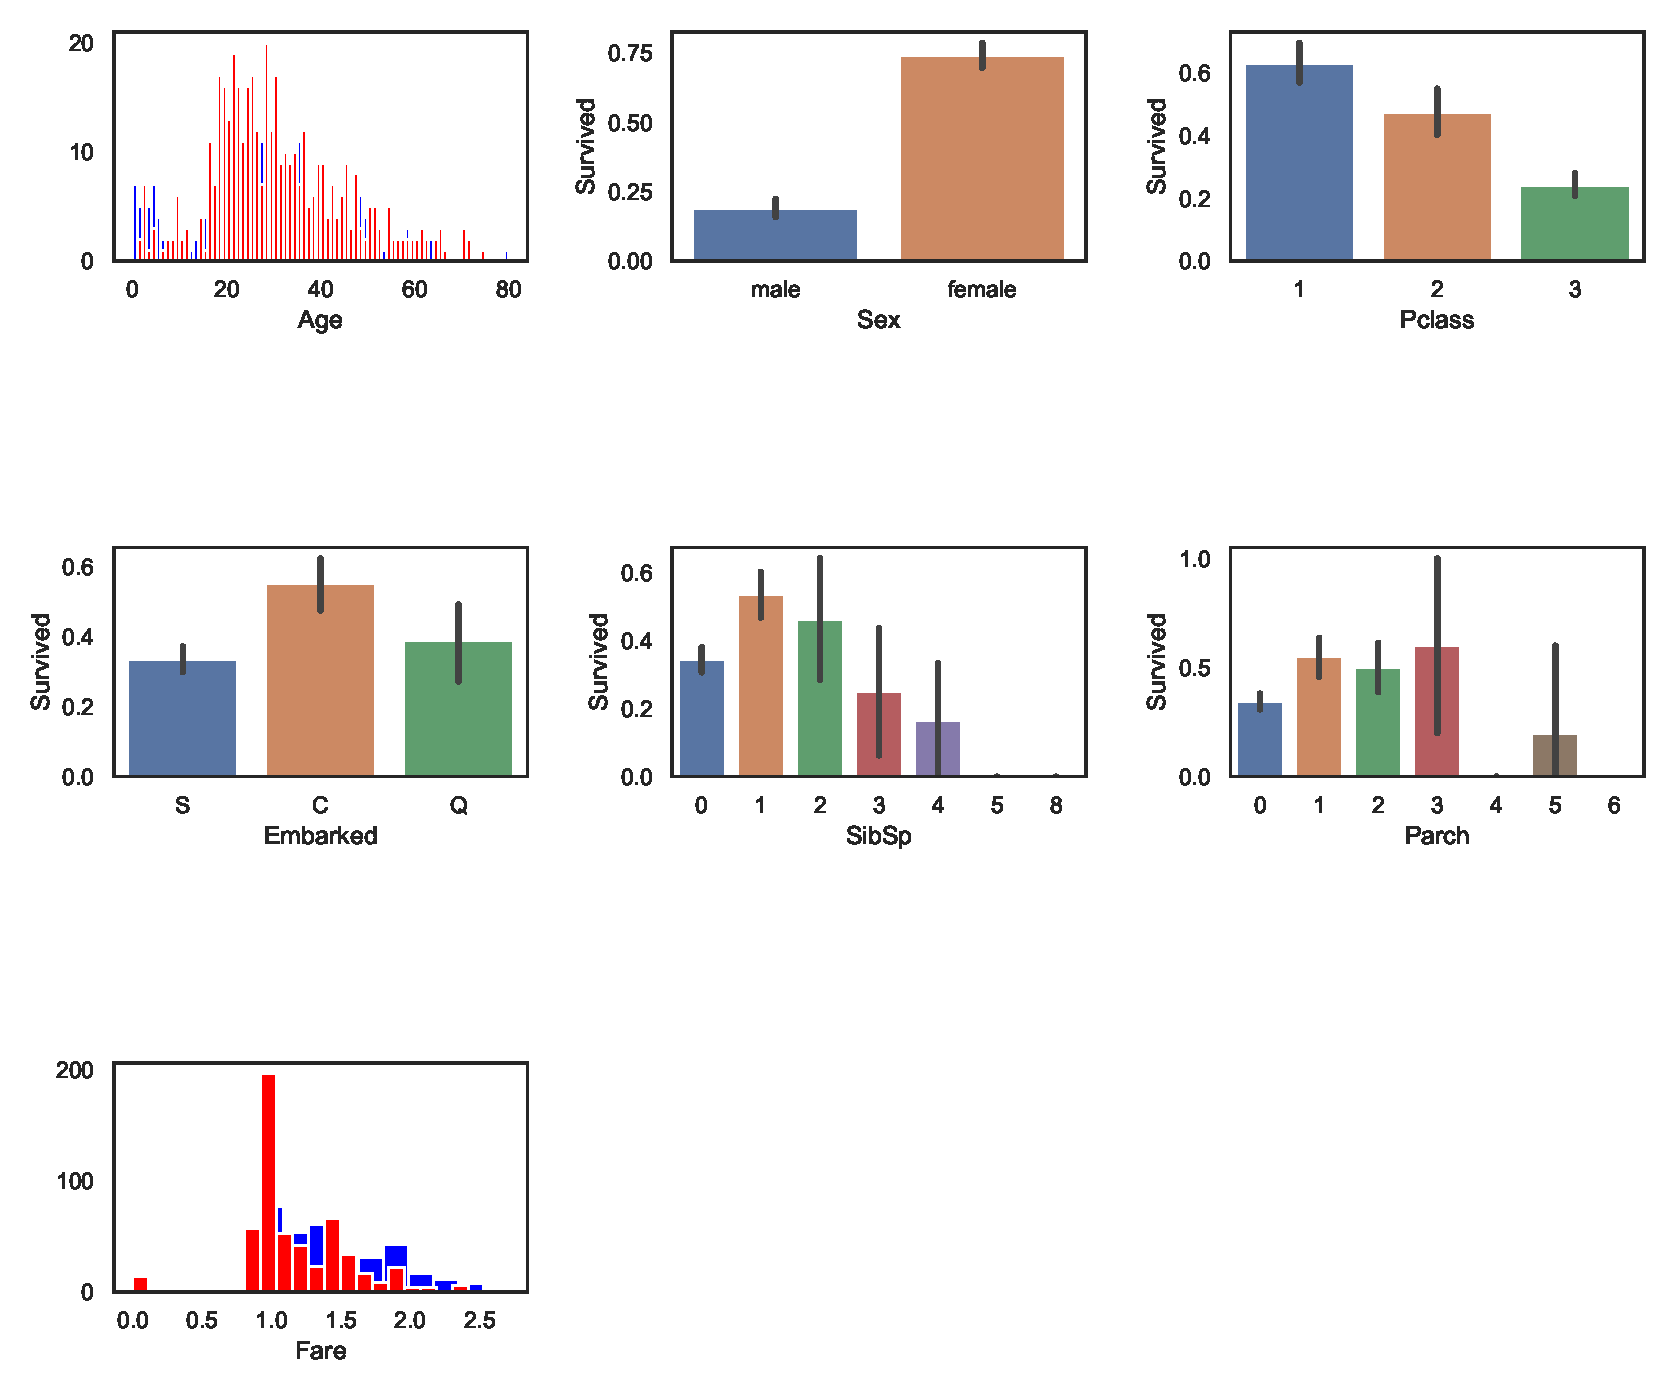
\includegraphics[width=1.0\textwidth,height=0.5\textwidth]{./graphics/titanicimg/allfeatures.eps}}
\end{figure}

\section{Observation of the Feature} \label{sec-analysis}
Sex: The chance of survival for women is high as compared to men.\\
  Pclass:There is a visible trend that being a 1st class passenger gives you better chances of survival. The survival rate for Pclass3 is very low. For women, the chance of survival from Pclass1 is almost 1 and is high too for those from Pclass2. Money Wins!!!.\\
  Age: Children less than 5-10 years do have a high chance of survival. Passengers between age group 15 to 35 died a lot.\\
  Embarked: This is a very interesting feature. The chances of survival at C looks to be better than even though the majority of Pclass1 passengers got up at S. Passengers at Q were all from Pclass3.\\
  Parch+SibSp: Having 1-2 siblings,spouse on board or 1-3 Parents shows a greater chance of probability rather than being alone or having a large family travelling with you.

\section{Correlation between the features} \label{sec-experiment}
\begin{figure}
  \centering
  %\selectcolormodel{rgb}
  \centerline{\includegraphics[width=1.0\textwidth,height=0.5\textwidth]{./graphics/titanicimg/heatmap.eps}}
  \caption{Interpreting the heatmap}\label{fig:Heat map}
\end{figure}
Now from the above heatmap,we can see that the features are not much correlated. The highest correlation is between SibSp and Parch i.e 0.41. So we can carry on with all features.
\section{Feature Engineering and Data cleaning} \label{sec-datacleaning}
The next idea is to define new features based on the existing ones that allow for a split into survived/not-survived with higher confidence than the existing features.
Some of the features like Age is converted into suitable form like Age-Band for modeling. This part of the analysis is called Feature Engineering
We need to convert the continuous values like age into categorical values by either Binning or Normalisation. It is necessary to remove redundant features like Name, Ticket, Fare, etc.
\section{Predictive Modeling} \label{sec-modeling}
We have gained some insights from the EDA part. But with that, we cannot accurately predict or tell whether a passenger will survive or die. So now we will predict the whether the Passenger will survive or not using some great Classification Algorithms.\\
Our problem is a classification and regression problem. We want to identify relationship between output (Survived or not) with other variables or features (Gender, Age, Port...). We are also perfoming a category of machine learning which is called supervised learning as we are training our model with a given dataset. With these two criteria - Supervised Learning plus Classification and Regression, we can narrow down our choice of models to a few.\\
1)Logistic Regression\\
2)Support Vector Machines(Linear and radial)\\
3)Random Forest\\
4)K-Nearest Neighbours\\
5)Naive Bayes\\
6)Decision Tree\\
Total sample size = 623; training sample size = 623, testing sample size = 268\\
\begin{table}  \centering
  \caption{Accuracy Comparison of different Classifier Algorithms}
  \label{tbl:overall-experiments}
  \begin{tabular}{cccc}
\toprule
    % after \\: \hline or \cline{col1-col2} \cline{col3-col4} ...
     & Acuracy \\
\midrule
    Radial Support Vector Machines(rbf-SVM)   & 0.835820895522388 \\
    Linear Support Vector Machine(linear-SVM) & 0.8171641791044776 \\
    Logistic Regression & 0.8134328358208955 \\
    Decision Tree & 0.8059701492537313 \\
    K-Nearest Neighbours(KNN) & 0.832089552238806 \\
    Gaussian Naive Bayes & 0.8134328358208955 \\
    Random Forests & 0.8208955223880597\\
\bottomrule
\end{tabular}
\end{table}

\section{Conclusions} \label{sec-conclusions}
This is only the basic modeling of the data. The results can be further enhanced. To overcome the model variance, and get a generalized model,we can use Cross Validation.



